\chapter{Alternate Methods}
\label{sec:Prior Works}
Currently, FMRI is used to determine the location of responses
to stimuli. The method of finding activation is discussed in 
\autoref{sec:Statistical Parametric Mapping}. The goal of this 
work is to move away from simple localization, and move toward
characterizing the response curve. Doing so 
necessitates more complex models and requires
more computation. Already there have been several other
attempts to model the BOLD response; these works will be discussed
in this chapter.

\section{Statistical Parametric Mapping}
\label{sec:Statistical Parametric Mapping}
Although not strictly the same as parameter calculation from 
FMRI, activation detection is similar and worth discussing. Estimation of 
parameters is a generalization of the idea 
of activation detection.
Given the popularity of Statistical Parametric Mapping (SPM) 
it is important to draw a distinction between it and the methods proposed
in this work.

\subsection{Random Field Theory}
\label{sec:RFT}
SPM methods make significant use of $t$-Tests across large regions;
however, such $t$-tests work slightly differently than a single
individual test. A $t$-test with a p-value of $0.05$ over 
10,000 voxels, will on average generate 500 false
positives. This is called the multiple comparison problem. Traditional
Bonferroni Correction
deals with this by requiring each test to pass with P
value of $\frac{0.05}{10000}$. The probability of 
a single false positive would then be $0.05$. Unfortunately this leads to unrealistically
low p-values; so low that it would be impossible for any biological system to satisfy. To
compensate, a Gaussian kernel is applied to smooth the image. This has
the benefit of reducing the noise variance and 
decreasing the effective number of independent measurements. Because
the number of \emph{independent} measurements is smaller, Bonferroni correction
can theoretically be applied with a lower scaling factor than
the original voxel count \cite{Worsley2004}. As side effect of this 
extreme smoothing, a single voxel activation is very hard to detect.

\subsection{Classical Activation Detection}
\label{sec:Square Wave}
The most basic method of analyzing FMRI data is by standard $t$-test
between resting state and active state samples. Simply put, the
mean is calculated separately for non-stimulus and stimulus time intervals.
A classic $t$-test may then be applied, giving the probability that the
distributions actually have the same mean. Because of the correlated
noise present in FMRI (\autoref{sec:Introduction Noise}), it is necessary
to apply a high-pass filter to the data. Without applying
such a filter, P values must be set extraordinarily high to prevent
false positives \cite{Smith2007}. Because the BOLD response is known
not to fit a square wave this method is rarely used
(\autoref{sec:BOLD Physiology}). For this reason other methods
are often more used, as discussed in 
\autoref{sec:Current Techniques General Linear Model}.

\subsection{General Linear Model}
\label{sec:Current Techniques General Linear Model}
The most common FMRI analysis tool is SPM, which generates
statistical parametric map using more advanced methods than a simple
square wave. Hierarchal
Models are one important improvement that allows researchers
to combine data across multiple runs, patients and stimuli
(see \cite{Hofmann1997} for more on Hierarchical Modeling). 
Hierarchical Models
concatenate all the data into a single dataset, then perform
a linear fit between a design matrix and the data. The design matrix
encapsulates all known experimental factors such as stimuli,
young/old, etc.  The general linear model is defined as:

\begin{equation}
Y(t) = X(t)\beta + \epsilon(t)
\end{equation}

where $Y(t)$ is the smoothed or de-trended time course of measurements,
$X(t)$ is the design matrix, $\beta$ is a column vector of weights,
and $\epsilon$ is the error. Thus for every time, the measurement is
assumed to be a weighted sum of the columns of $X$ plus some error. The calculation
of $\beta$ is then performed using a maximum likelihood or gradient descent search 
to minimize the error. 

\begin{figure}
\centering
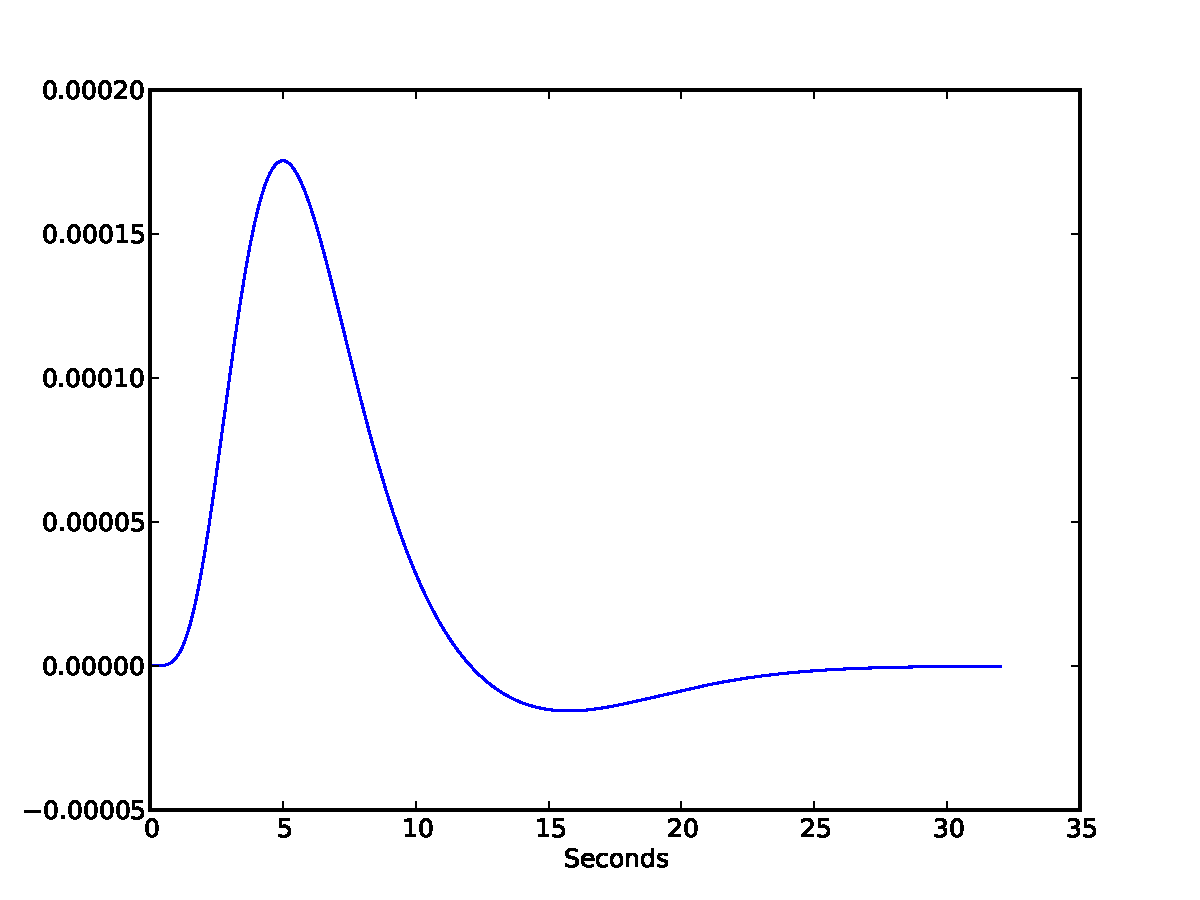
\includegraphics[scale=.7]{images/HRF}
\caption{Canonical Hemodynamic Response Function (y-axis units are arbitrary because 
normalization is performed).}
\label{fig:HRF}
\end{figure}

As mentioned previously, a square wave stimulus 
does not result in a square wave in the activation of brain regions. 
The BOLD signal is in fact a smoothed version of the 
stimuli. As such, when fitting an FMRI time course to the input,
the input ($X$'s columns) is usually smoothed to reduce bias error. 
The best method, that maintains a linear fit, is convolving the input 
with a Hemodynamic 
Response Function (HRF). The \emph{Hemodynamic Response Function}
mimics the basic shape of BOLD activation, including a delay
due to rise time and fall time. The fitting 
process is then a least squares fit over the space of the vector $\beta$. 
Therefore $Y(t)$ is estimated as a linear combination 
of the columns of $X$. 

Smoothing the input with a single HRF poses certain problems.
It is well known that different Hemodynamic Response Functions are necessary 
for different regions of the brain \cite{Handwerker2004}. The Canonical HRF that is most often used, 
has been optimized for the visual cortex. As discussed in \autoref{sec:Post Stimulus Undershoot},
there are definitely variations in the shape of the
BOLD response, over both brain regions and patients. Handwerker et. al. 
discussed the implications of choosing an incorrect HRF, the most important
of which is a definite increase in false negatives \cite{Handwerker2004}. While an atlas
of Hemodynamic Response Functions for each region could definitely 
mitigate this risk, it does not account for variation between patients.

\subsection{Hierarchical Linear Models}
As mentioned previously and discussed extensively
in Friston et al. and Hoffman et al., hierarchical models may be 
applied to account for systematic differences between subjects
\cite{Friston2002, Hofmann1997}. For instance, if the
study mixes young and old, incorporating
that into the model is wise, regardless of whether it is the goal of the test. 
The reason to do this is to account for additional variance that may not
be otherwise explainable.  The Hierarchical form used by
Friston et al. is shown in \autoref{eq:Hierarchical} \cite{Friston2002}.

\begin{eqnarray}
\label{eq:Hierarchical}
Y(t) & = & X_1(t)\theta_1 + \epsilon_1(t)            \nonumber \\
\theta_1(t) &=& X_2(t)\theta_2 + \epsilon_2(t)     \nonumber \\
 & ... &                                             \nonumber \\
\theta_{n-1}(t)& =& X_n(t)\theta_n + \epsilon_n(t) 
\end{eqnarray}

The Empirical Bayes algorithm was used by both Friston et al. and Hofmann et al. 
\cite{Friston2002, Hofmann1997}. Note that in Empirical Bayes point estimators 
are used for each $\theta$, rather than full distributions or the first two moments.

\subsection{Discussion}
\label{sec:BackgroundConclusion}
In all, the GLM is useful for determining linear 
dependence of a set of regressors on the output. Unfortunately, as discussed in
\autoref{sec:BOLD Analysis} there are significant nonlinearities 
that almost certainly cause false negatives in the Statistical Parametric
Maps. Unfortunately nonlinear analyses have only recently become feasible,
so the scale of the problem is still unknown. The problem is 
highlighted by the common scenario where no significant
activation can be found in a single run \cite{Riera2004, Johnston2008}.  

The static nature of the  linear model also limits its potential use. 
Besides not allowing HRF differences between patients, there is no
reasonable way to incorporate other forms of physiological
data. Combined FMRI CBF or CBV imaging methods are improving,
as seen in Chen et al. \cite{Chen2009}. These techniques could shed light on
neural activation by providing extra measurements, yet a 
physiologically reasonable model is necessary to incorporate this extra data.
Activation detection methods also don't have the ability 
to identify pathologies based on state variables or parameters. For
example, decreased compliance of
blood vessels could indicate, or even cause, a neurological condition that 
is not easily seen in other imaging modalities. 

\section{Approaches to the Balloon Model}
Unlike Statistical Parametric Mapping, the techniques described in this
section are all attempts to regress some version of the BOLD model. 
Although Buxton et al. and Friston et al. 
both proposed physiologically reasonable values for the model parameters, 
Friston et al. in 2002 was the first paper to calculate the parameters based 
on actual FMRI data \cite{Buxton1998, Friston2000, Friston2002b}. 
However, in that case, the voxels were chosen from
regions that were detected as active by the GLM. It is therefore possible
that the parameters are biased toward parameters that fit the linear model.

\subsection{Polynomial Approximation}
\label{sec:Background Linear Approximation}
In Friston et al., a novel combination of linear and nonlinear modeling
was used to generate parameter estimates \cite{Friston2002b}. 
Although this method was restricted to regions determined to be 
active by the GLM, there is no reason it could not be applied more broadly.
Because there is no closed 
form solution to the balloon model, it impossible to 
calculate the Jacobian matrix $\frac{\partial Y}{\partial \theta}$. Thus 
Friston et al. approximated the partial using a Volterra Kernel \cite{Friston2002b}. 
At each step of the Expectation-Maximization (EM) algorithm, 
the differential equation was integrated and the residuals
calculated. Then, for each $\theta_i$ surrounding the estimate of 
$\theta$, a Volterra-Kernel expansion of the output $y$ was generated. Generation
of the Volterra Kernel is quick, and, since there
is an analytical solution, calculating partial derivatives is easy. 
The full E-M algorithm for estimating the states is notation-heavy 
 and can be found in Friston et al. \cite{Friston2002b}.

There are a few caveats with this method of optimization. First, the 
partials are based on an approximate values (using Volterra-Kernels) of $y$.
Importantly, the Volterra-Expansion of $y$ is not able to model interactions
between state variables; which certainly increases error \cite{Friston2002b}.
Additionally, to date no extensive review of the accuracy of the 
Volterra expansion has been performed. Finally all the tests performed
by Friston et al. were on regions found to be active by the General
Linear Model \cite{Friston2002b}. For this reason, the reliability of 
the approximation is unknown for regions that are active but sufficiently 
nonlinear to avoid detection by conventional tests.

\subsection{Nonlinear Least Squares}
\label{sec:Nonlinear Least Squares}
Although there are certainly benefits to using a derived model, rather
than a purely empirical model, there are serious implications. The
first problem is that all the powerful linear techniques of gradient
descent are off limits; since the model is a true nonlinear dynamical
system with no closed form solution (although \autoref{sec:Background Linear Approximation}
circumvented this by calculating a Volterra Series approximation). Without
a Jacobian for residuals, the Gauss-Newton method
is impossible. Additionally, a gradient descent is slow
without the ability to form partials of the output with respect
to all the parameters. 

Still, there are other heuristic algorithms
that could illuminate the BOLD response. 
Simulated Annealing (SA) is a common method of optimizing high dimensional
regression problems. First the program selects a random starting point, then
at each iteration it selects a random point in the neighborhood. If the 
new point is 
below some energy constraint (energy is a function of the residual), 
called the temperature, the algorithm moves
to that point and continues with the next iteration. The temperature
is slowly lowered until no nearby points below the temperature can
be found. There are
variations of this, for instance it is common to require every movement
to be in the downward direction (in terms of energy). Like most nonlinear
optimization problems, there is no guarantee of an optimal solution,
although the longer the algorithm is allowed to run, the better the solution.
Since every step requires a re-integration of the  
balloon model, it can be extremely time consuming, which is why I did 
not use it here.

\begin{algorithm}
\caption{Simulated Annealing Algorithm}
\label{alg:Simulated Annealing}
\begin{algorithmic}
\STATE Initialize $\Theta$, or if there exists a decent estimate start there
\STATE Initialize temperature, T to value above initial energy
\WHILE{$E(\Theta) < T$}
    \REPEAT
        \STATE Pick $\theta$ near $\Theta$
        \STATE Calculate energy, $E$, of $\theta$
    \UNTIL{$E > T$}
    \STATE Move to new estimate: set $\Theta = \theta$
\ENDWHILE
\end{algorithmic}
\end{algorithm}

Genetic algorithms (GA) are similar to Simulated Annealing, in
that they randomly move to better solutions based on a cost function.
However, in genetic algorithms, a single point estimate isn't used. Instead
a population of estimates is generated, each with distinct parameters,
and then each set of parameters is rated with a fitness function. Parameter
sets that are good get a higher weight. New parameter sets are generated by 
randomly combining pieces of the old parameter sets. The pieces are 
chosen at a rate proportional to the fitness of the donor; thus good
parameter sets tend to pass on their properties. In addition to this,
random mutations are introduced that come from no existing parent. 
The fitness function is then used to weight the new generation, and
the entire process starts over. The stop condition for a genetic algorithm
is typically based on some threshold for fitness or a maximum number 
of generations. As with simulated annealing (or any generic non-linear optimization),
there is no guarantee that a global minimum has been reached.

\begin{algorithm}
\caption{Genetic Algorithm}
\label{alg:Genetic Algorithm}
\begin{algorithmic}
\STATE Initialize $N$ estimates, $E = \{\Theta_0, \Theta_1, ... \Theta_N\}$
\FOR{G generations}
    \STATE Calculate fitness for each $\Theta$, Ex. for residual $R$, $1/R$ or, $e^{-R}$
    \FOR{$i$ in $N$}
        \STATE Randomly select two parents (with higher probability for more fit $\Theta$'s)
        \STATE Randomly merge parts of the two parents to form a new $\Theta_i$
        \STATE With low probability introduce random mutations to parameters in $\Theta_i$
    \ENDFOR
\ENDFOR
\end{algorithmic}
\end{algorithm}

Although both these methods can be highly effective, they have the downside of
requiring high computation time. In the case of the BOLD model,
each time the energy or fitness needs to be calculated, a large number of cycles
must be spent re-simulating the BOLD model for the set of parameters. As I'll
discuss in \autoref{sec:Particle Filter}, the Particle Filter method is able
to circumvent this re-calculation to some degree. Its worth noting though, that 
to beat the particle filter algorithm discussed in \autoref{sec:Particle Filter} 
these would have to converge in less than 1000 simulations (which is far less than
1000 generations in GA). 

\subsection{Unscented Kalman Filter}
\label{sec:Unscented Kalman Filter}
The Unscented Kalman Filter (UKF) is a powerful Gaussian/Bayes filter that attempts
to model the posterior distribution of dynamical systems as a multivariate
Gaussian. The Unscented Kalman Filter (UKF) generalizes the Extended Kalman
Filter by allowing the state update and output functions to be arbitrary functions.

\begin{eqnarray}
X(t) &=& g(u(t), X(t-1))\\
Y(t) &=& h(X(t))
\end{eqnarray}

In order to estimate the posterior at $t$, a deterministic set of sigma points 
(often 2 per dimension, plus 1 at the mode of the multivariate distribution)
weighted according to a Gaussian estimate of $X(t-1)$ are passed through
the update equation. This set of points are then used to estimate the 
mean and covariance of $X(t)$. The benefit of this is that it requires
no Jacobian and only a few extra calculations to get a decent estimate of
a posterior Gaussian. Hu et. al. used the UKF to  perform a similar type of analysis to
the one performed in this work \cite{Hu2009}. 

\begin{figure}
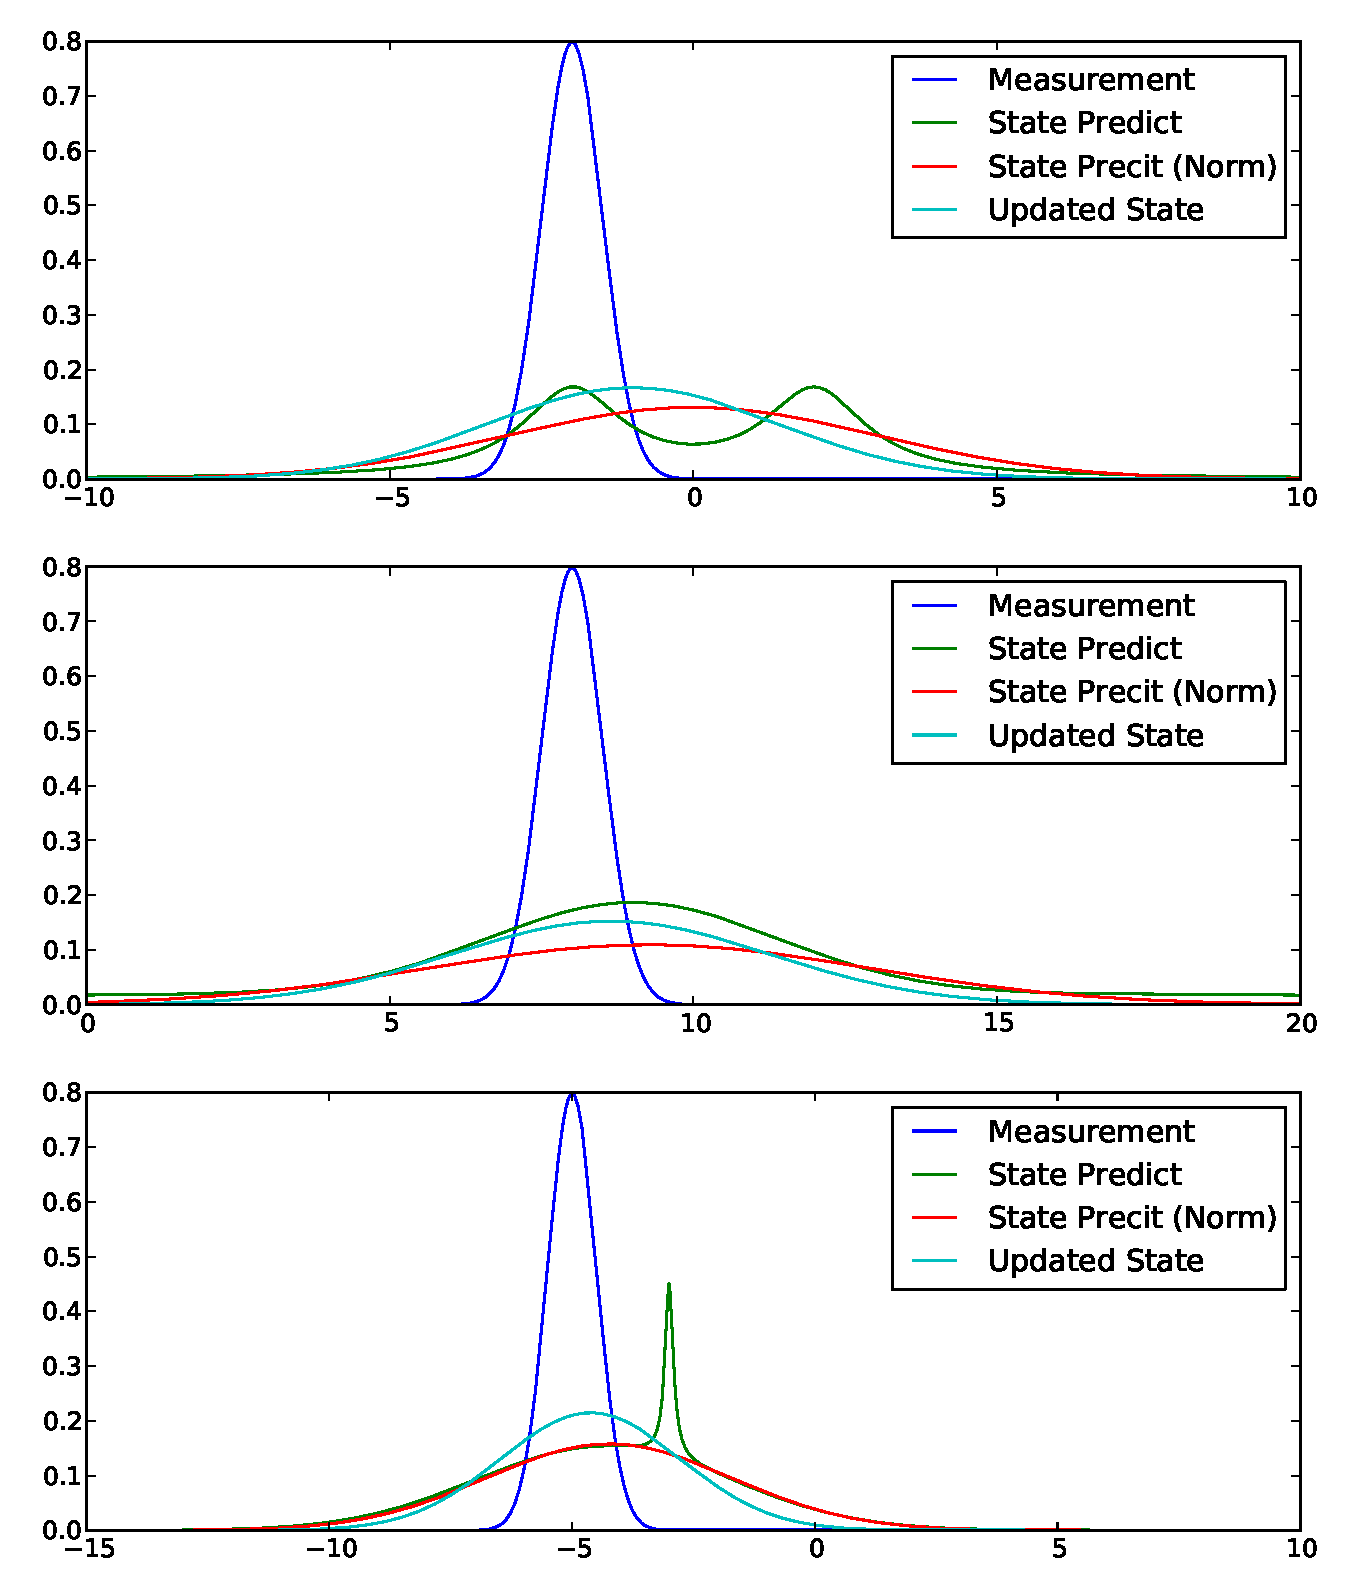
\includegraphics[width=16cm]{images/kalman}
%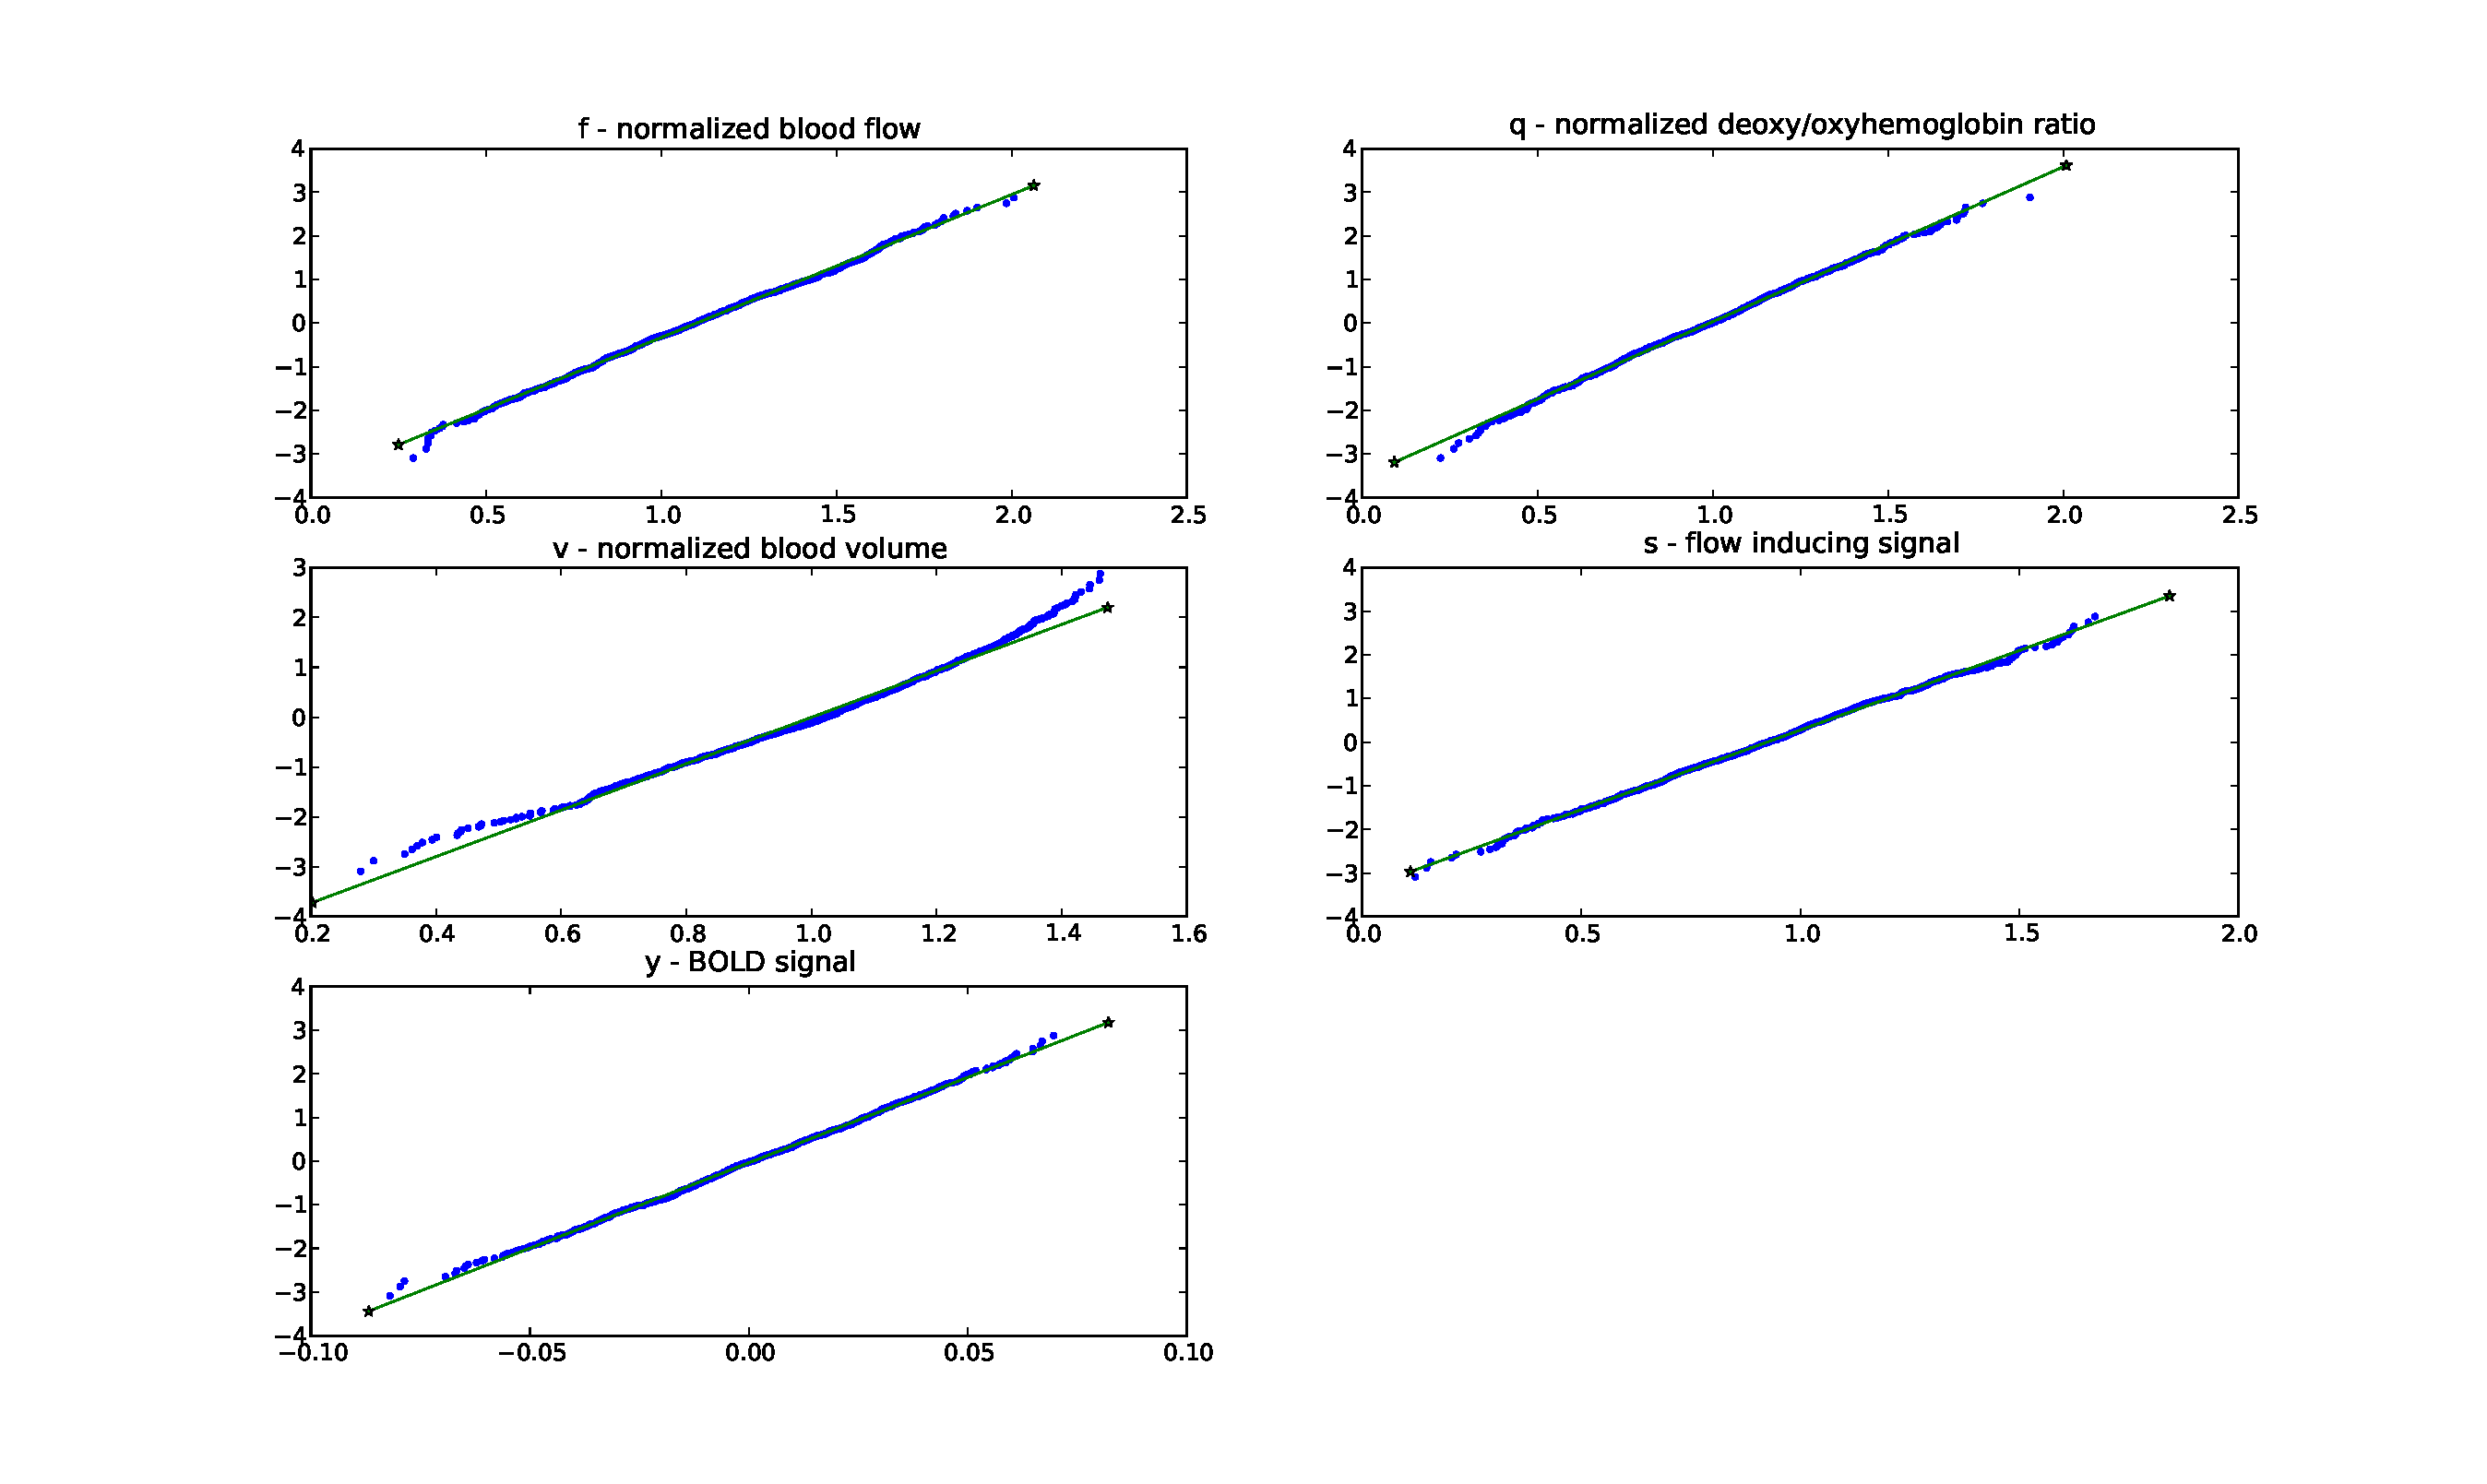
\includegraphics[trim=6cm .75cm 6cm .75cm,width=16cm]{images/gauss_step_point1sec_3sigma.pdf}
\caption{Example updates of a distribution using the Kalman Filter.}
\label{fig:EKFWorking}
\end{figure}

The difficulty
of using a Kalman Filter, however, is that it assumes a multivariate 
Gaussian for the state variables, $X(t-1)$. The more nonlinear the system
gets the more likely that the Gaussian will be insufficient to describe
the distribution, $X(t)$. When this occurs, every step from  $X(t+1)$ 
to $X(t)$ will introduce additional
error in the posterior distribution. Furthermore, it is not really known what 
sort of underlying distributions may exist in such a mixed biological,
mechanical, chemical system such as the brain.
 The assumption of Gaussianity is what allows
the UKF to estimate the posterior using only the first and second moments;
however, if this assumption is violated significant error will result.
 On the other hand, for
small variances and short time steps the Gaussian distribution is a good 
fit, and so in some cases the Unscented Kalman Filter could work quite
well. 
\begin{table}[t]
\centering
\begin{tabular}{|c || c |}
\hline 
Parameter & Run 1 \\
\hline
$\tau_0$ & .98  \\
$\alpha$ & .33 \\
$E_0$ & .34  \\
$V_0$ & .03  \\
$\tau_s$ & 1.54  \\
$\tau_f$ & 2.46  \\
$\epsilon$ & .54  \\
$V_t$ & N(1, .09)  \\
$Q_t$ & N(1, .09)  \\
$S_t$ & N(1, .09) \\
$F_t$ & N(1, .09) \\
\hline
\end{tabular}
\caption{Parameters used to test Gaussianity of variables after being transitioned through
the BOLD model}
\label{tab:steptable} 
\end{table}

To determine the amount of error incurred in a Gaussian estimate during
a typical sample period, I assigned the states of BOLD equations according
to a four dimensional Gaussian. I then propagated the states through 
two seconds of simulation (a typical TR in FMRI) and plotted the resulting
marginal distributions against a Gaussian distribution. This also demonstrates
the degree of nonlinearity present in the system. The parameters used are 
shown in \autoref{tab:steptable}

In order to drive the system without input I intentionally set $s_t$ a non-steady
state, but physiologically plausible, value. The value of $u$ was left at zero 
the entire time, so the 
system would decay naturally (see \autoref{sec:BOLD Physiology})
\autoref{fig:transp1s} shows the results after the
system ran for 100 milliseconds. 
The Q-Q plots fit will with a Gaussian, demonstrating that at this short
time interval nonlinearities have not yet begun to effect the distribution.
However, \autoref{fig:trans1s} shows the result after 1 second, which is faster
than most FMRI scanners are capable of sampling at. At that range the tails 
of the distributions for $v$ and $q$ started to deviate from the
Gaussian distribution. As a result the uncertainty in $y$ deviated from
the Gaussian distribution as well. This is important, because although 
approximating the distribution with a Gaussian based on the first two
moments will worked in the short run, within a period less than typical
measurement rates the distribution deviated from a Gaussian substantially. 

Thus, even without introducing variation in the model parameters,
a distinct nonlinearity and non-Gaussianity was present. 
More advanced tests where parameters (especially $\alpha$) are varied
would certainly introduce more error into the Gaussian estimate. 
For this reason, estimating the posterior distribution using only 
the first two moments, which is the basis for the UKF, is not wise. 

\begin{figure}
\centering
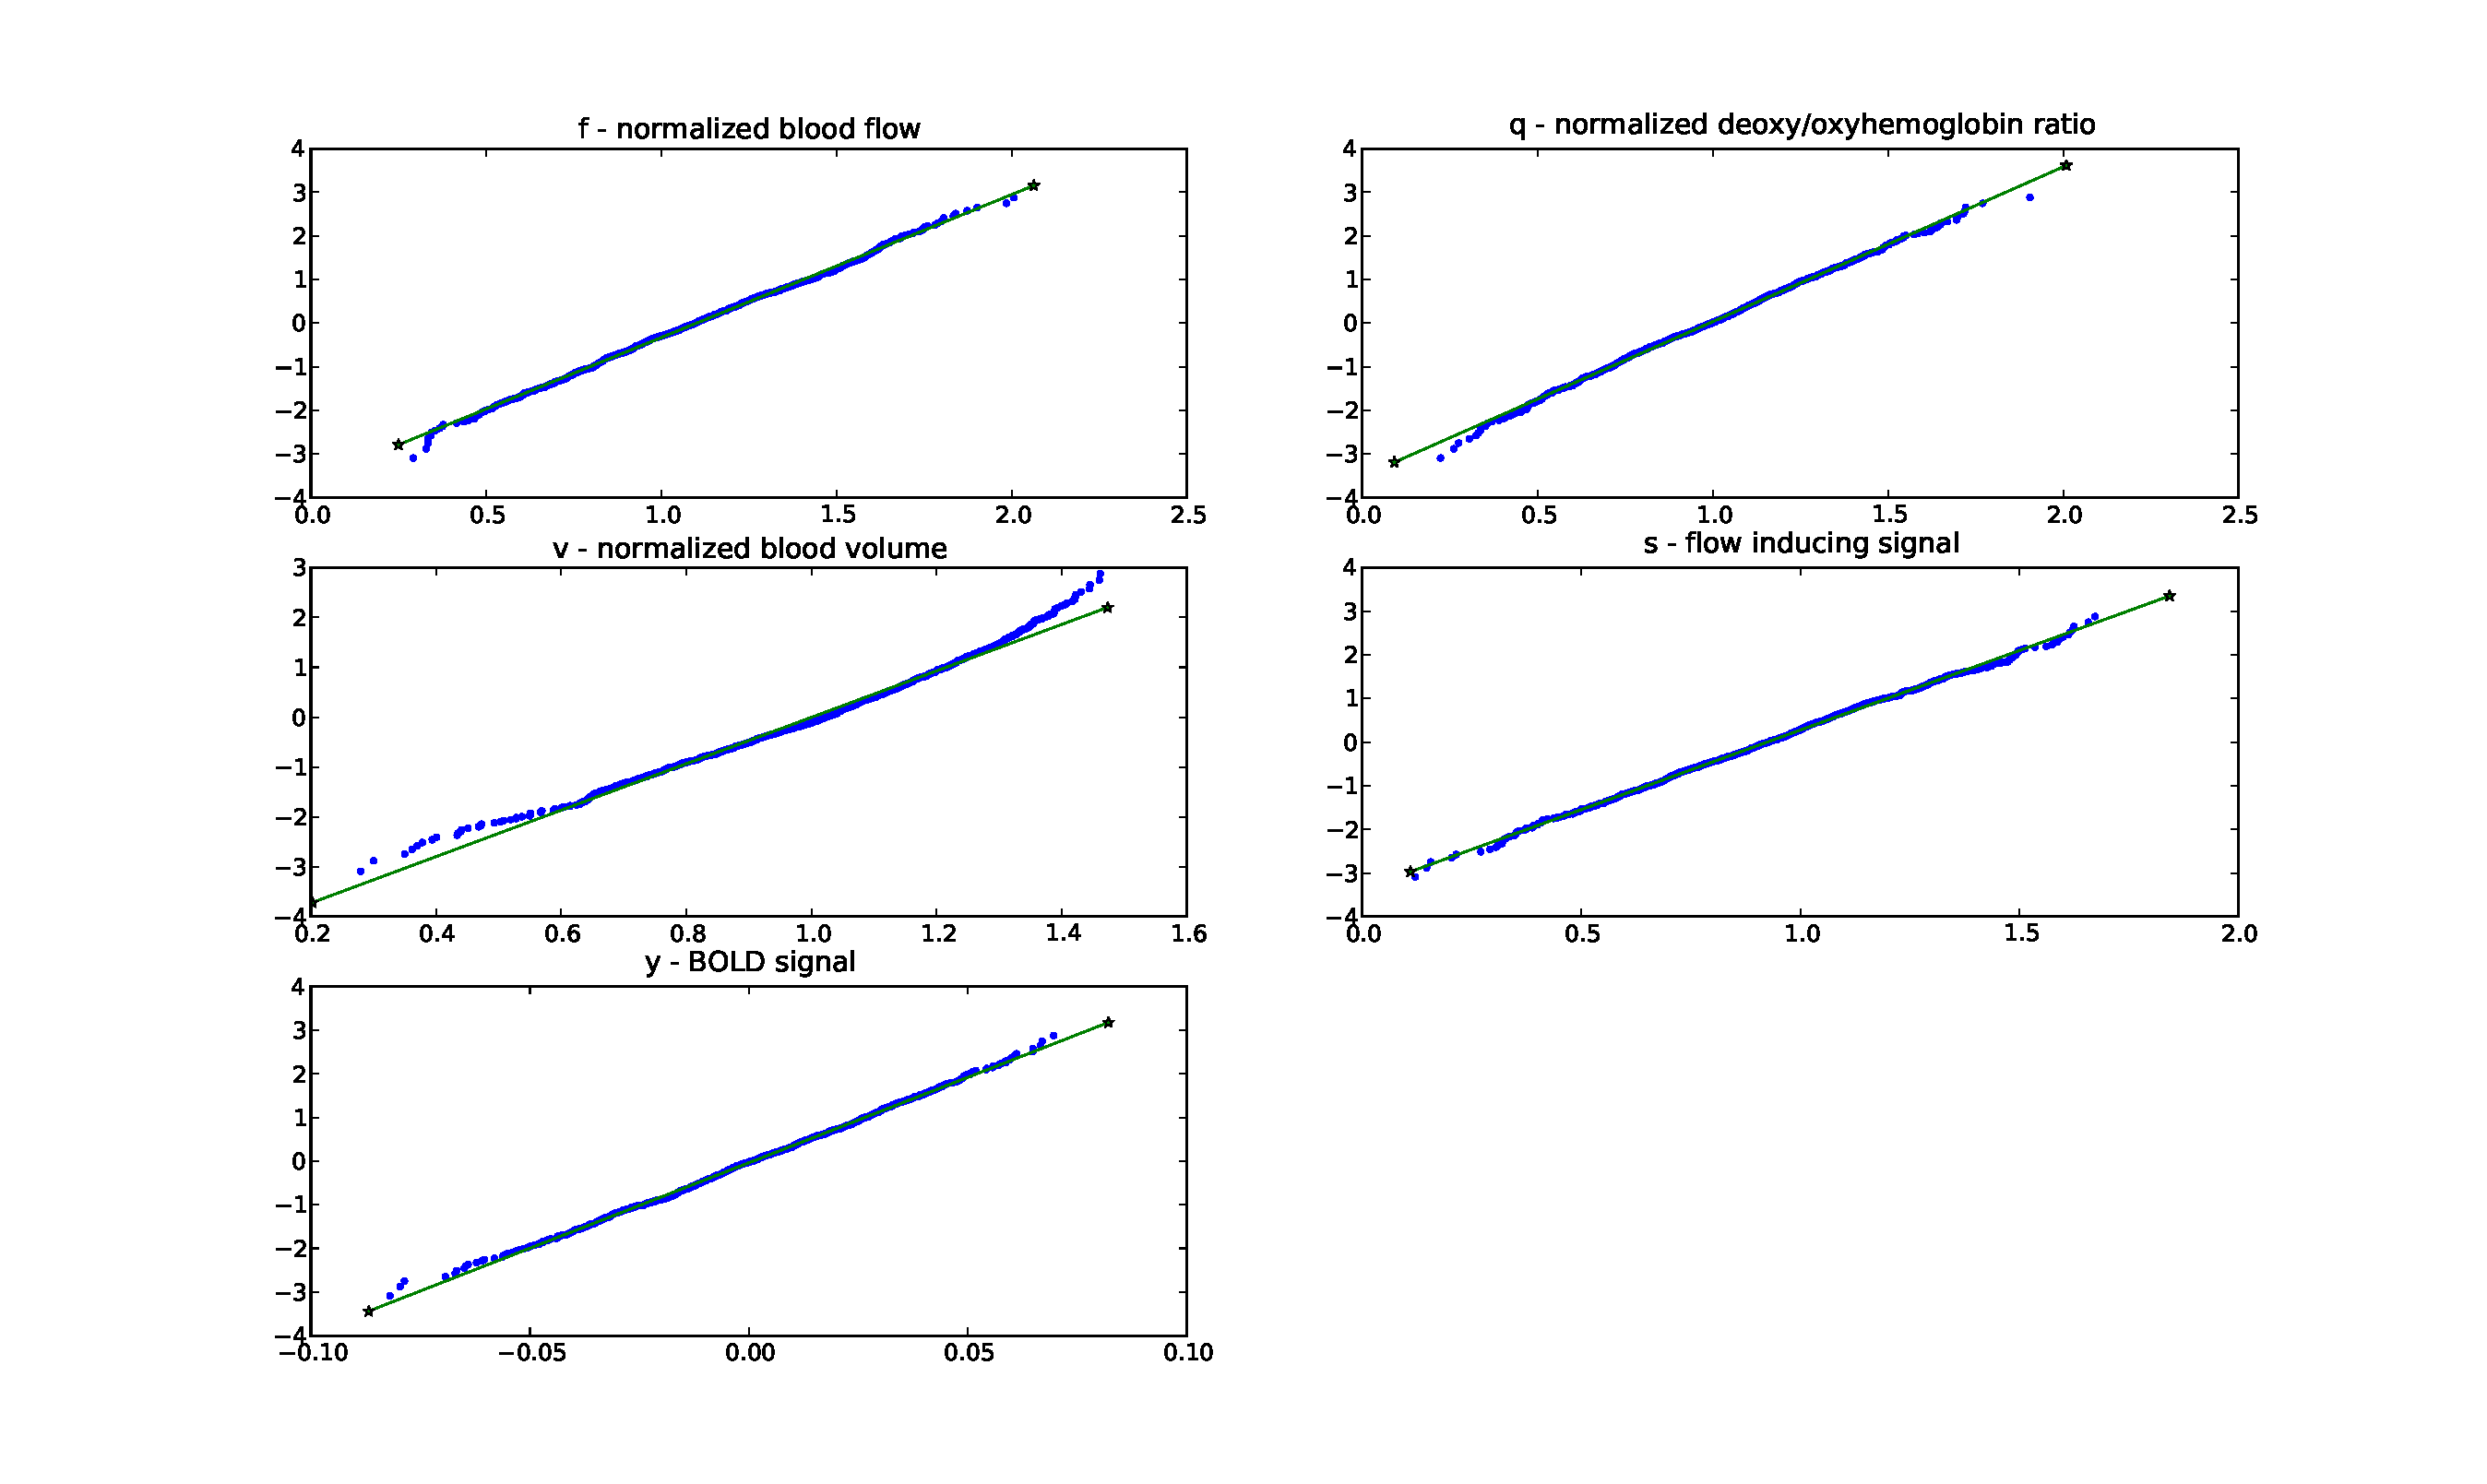
\includegraphics[trim=6cm .75cm 6cm .75cm,width=16cm]{images/gauss_step_point1sec_3sigma.pdf}
\caption{Distributions of state variables after simulating for $0.1$s}
\label{fig:transp1s}
\end{figure}

\begin{figure}
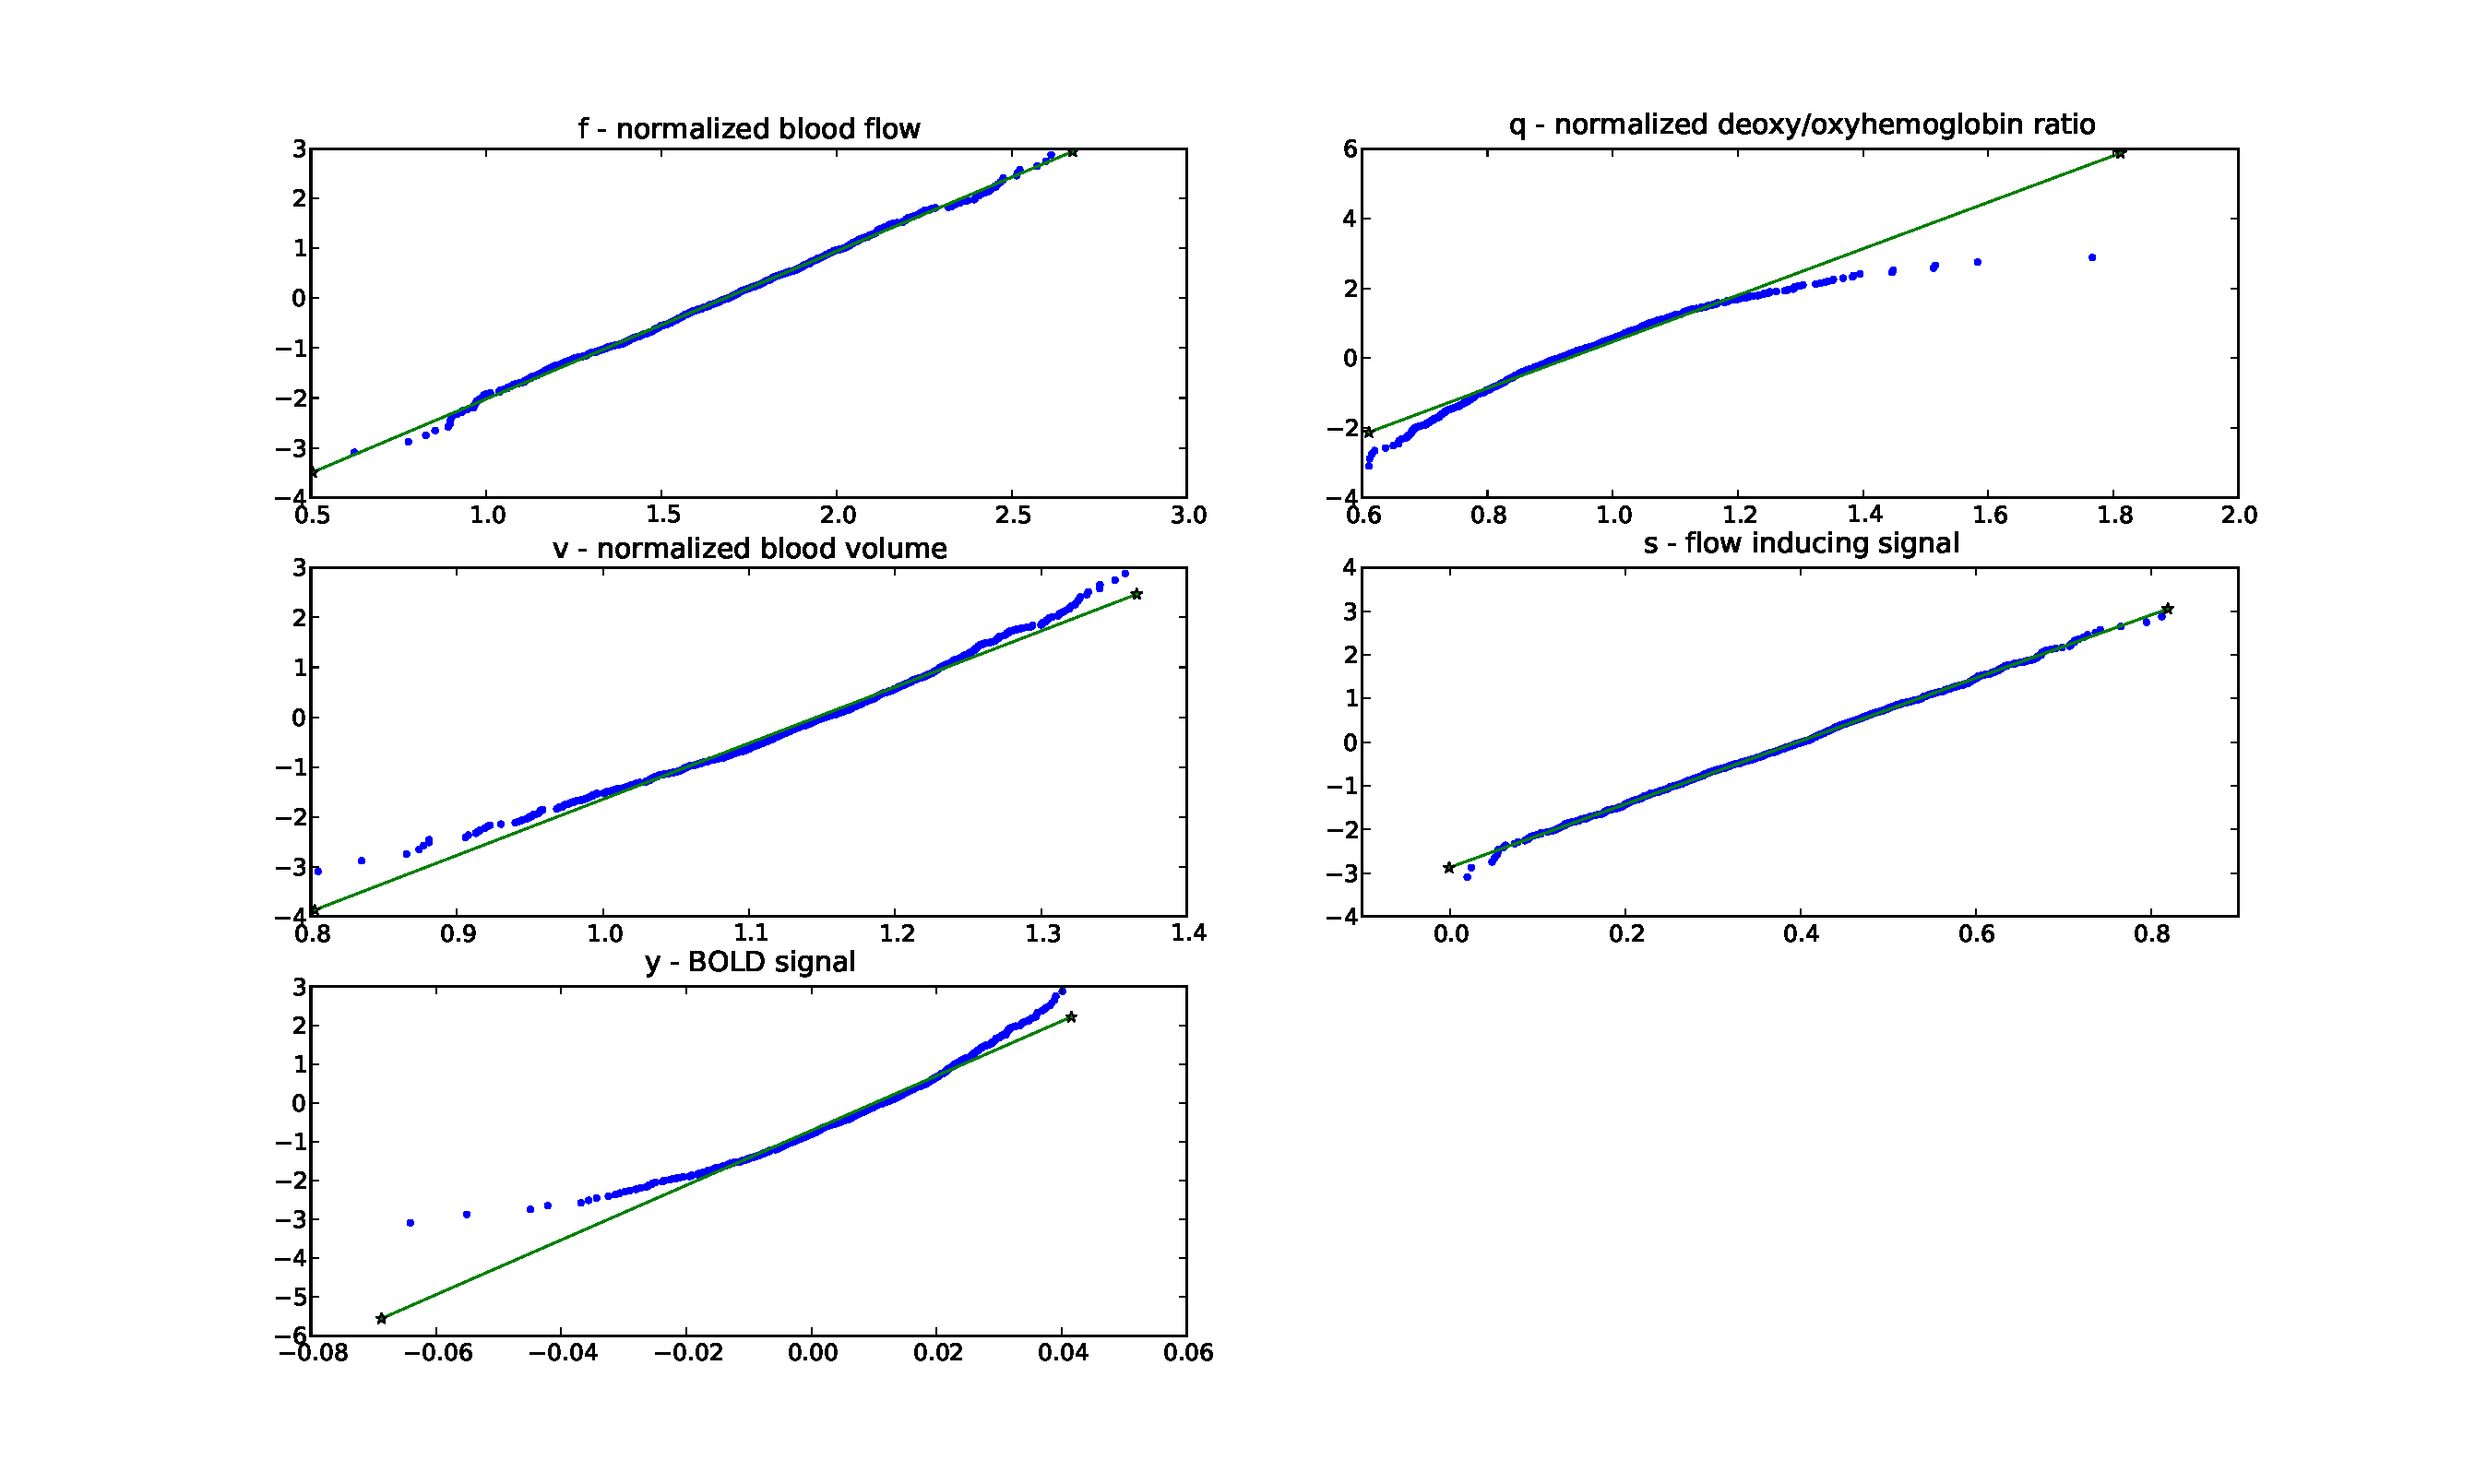
\includegraphics[trim=6cm .75cm 6cm .75cm,width=16cm]{images/gauss_step_1sec_3sigma.pdf}
\caption{Distributions of state variables after simulating for $1$s}
\label{fig:trans1s}
\end{figure}

\subsection{Hybrid Methods}
In Riera et al. , a maximum
likelihood method for innovation processes was used, as described by
Ozakai \cite{Riera2003,Ozaki1994}. Ozaki used a similar construction to a 
Kalman filter on nonlinear signals \cite{Ozaki1994}. 
The method used by Riera et al. used this method to perform maximum likelihood on
the innovations rather than the absolute signal levels \cite{Riera2003}. 
By using a Local Linearization Filter,
innovation noise such as noise in $\dot{f}$ is turned into simple 
Gaussian noise. This approach is useful when the DC portion of the signal is
of no use; however, it depends greatly on the type of signal. I found that
this method was not very effective for the BOLD signal, when I used it 
with the particle filter approach discussed in the next chapter; although its
effectiveness depended greatly on the stimulus.

In Johnston et al., a hybrid particle filter/gradient
descent algorithm was used to simultaneously derive the static and dynamic 
parameters, (classically known as parameters and state variables, respectively)
 \cite{Johnston2008}.
A particle filter was used to calculate the state variables at each
time; then the estimated distribution of the particles was used to find
the most likely set of parameters that would give that distribution of state variables.
This process was repeated until the parameters converged. Interestingly Johnston et al.
came to a very different set of parameter estimates as compared
to the original Friston et al. estimates (\autoref{tab:Params})
\cite{Johnston2008, Friston2000}. In fact the results 
are significantly different from virtually every other study. The most obvious discrepancy
is the larger time constants, $\tau_f$, $\tau_s$ and $\tau_0$. 
While of course this could be poor convergence of the algorithm, there is another other possibility.
Unlike all the other methods mentioned, excepting the methods in \autoref{sec:Nonlinear Least Squares},
the algorithm described in Johnston et al. does not depend on prior distributions \cite{Johnston2008}.
It is possible then that the bias toward the prior in other methods skewed their results. 
While Johnston et al. is certainly in the minority; further exhaustive studies 
of the parameters, using unbiased techniques may be called for \cite{Johnston2008}. A further 
comparison between the distributions found in Johnston et al. and Friston et al. 
will be discussed in \autoref{sec:PriorDist} \cite{Johnston2008, Friston2000}.

In Vakorin et al., a combination of Genetic Algorithms and Simulated Annealing were
used to estimate not only the parameters, but the true stimuli driving the BOLD
signal \cite{Vakorin2007}. 
This addresses the inherent uncertainty of exactly where and when 
stimuli actually get applied. Unfortunately this algorithm was extremely slow.

\subsection{Previous Particle Filter Approaches}
In a PhD thesis, Murray used a particle filter based approach was used to integrate
the BOLD equations \cite{Murray2008}. The method used in that work focused primarily on estimating
the BOLD output and state equations as a nonlinear stochastic differential 
equation. The primary difference between that work and this is that
Murray took the parameters as a given \cite{Murray2008}. Thus, differences in the BOLD output
were taken to be primarily driven by stochastic changes in the underlying state
equations. Because the parameters were not allowed to change, the estimate of 
the BOLD signal was not very good. The fact that the
differences in BOLD response cannot be explained solely by stochastic elements 
is important, however. The filtering framework created
in that work, dysii, forms the basis for the particle filter used in this work, 
and was very designed. The work also clearly presents the particle filter;
both its derivation and use. 

\section{Conclusion}
Currently there is no ideal solution to solving this system of nonlinear
equations. Exhaustive search type methods such as those employed by
Johnston et al. and Vakorin et al. have long
run times even for a single voxel \cite{Johnston2008, Vakorin2007}. 
While Volterra models are an interesting
solution,there have not yet been exhaustive tests to determine whether
such approximations work well throughout state space. The most promising
method of those reviewed here is the Kalman filter based method. It is
able to maintain a fast runtime while still approaching the solution.
The reliance on a Gaussian estimate to the true posterior distribution could
cause problems however. 
The particle filter method proposed in the next section bears a strong 
resemblance to the unscented Kalman filter; albeit without the Gaussian 
assumptions. 
